\documentclass[aspectratio=169,11pt]{beamer}

% Compile with XeLaTeX.
\usepackage{fontspec}
\usepackage{polyglossia}
\setdefaultlanguage{vietnamese}
\setsansfont{Latin Modern Sans}
\setmainfont{Latin Modern Roman}
\setmonofont{Latin Modern Mono}

\usepackage{graphicx}
\usepackage{booktabs}
\usepackage{array}
\usepackage{tabularx}
\usepackage{tikz}
\usetikzlibrary{arrows.meta, positioning, calc, shapes.geometric}

\graphicspath{{../document/}}

\usetheme{Madrid}
\usecolortheme{seahorse}
\setbeamertemplate{navigation symbols}{}
\setbeamertemplate{footline}[frame number]
\setbeamertemplate{caption}[numbered]

\definecolor{uitblue}{RGB}{0,86,145}
\definecolor{softgreen}{RGB}{32,132,99}
\definecolor{softred}{RGB}{182,72,72}
\definecolor{softamber}{RGB}{191,128,36}

\setbeamercolor{title}{fg=uitblue}
\setbeamercolor{frametitle}{fg=uitblue}
\setbeamercolor{structure}{fg=uitblue}

\newcommand{\code}[1]{\texttt{\small #1}}
\newcommand{\metric}[2]{\begin{tabular}{@{}c@{}}\Large\textbf{#1}\\[-1mm]\scriptsize #2\end{tabular}}

\title[SmartLock Fuzzy]{Hệ thống khóa cửa thông minh\\nhận diện khuôn mặt kết hợp Fuzzy Logic}
\subtitle{CE224.Q11}
\author[N. H. M. Chiến \and P. M. Chí \and N. L. M. Anh]{%
Nguyễn Hữu Minh Chiến -- 23520183\\
Phùng Minh Chí -- 23520179\\
Nguyễn Lê Minh Anh -- 23520063}
\institute[UIT]{Trường Đại học Công nghệ Thông tin -- ĐHQG TP.HCM\\[1mm]
Giảng viên hướng dẫn: ThS. Phạm Minh Quân}
\date{\the\year}

\begin{document}

\begin{frame}
    \titlepage
    \vspace{-7mm}
    \begin{center}
        
\includegraphics[height=1.35cm]{uit_logo.png}
    \end{center}
\end{frame}

\begin{frame}{Nội dung trình bày}
    \begin{columns}[T]
        \begin{column}{0.48\textwidth}
            \begin{enumerate}
                \item Bài toán và mục tiêu
                \item Kiến trúc hệ thống
                \item Pipeline xử lý ảnh
                \item Fuzzy logic decision
            \end{enumerate}
        \end{column}
        \begin{column}{0.48\textwidth}
            \begin{enumerate}
                \setcounter{enumi}{4}
                \item Tích hợp phần cứng
                \item Giao diện web
                \item Benchmark trên thiết bị edge
                \item Kết luận và hướng phát triển
            \end{enumerate}
        \end{column}
    \end{columns}
\end{frame}

\begin{frame}{Bài toán}
    \begin{columns}[T]
        \begin{column}{0.56\textwidth}
            \begin{itemize}
                \item Khóa cơ, thẻ từ và mã PIN dễ mất, lộ hoặc bị sao chép.
                \item Nhận diện khuôn mặt giúp thao tác tự nhiên hơn, nhưng chất lượng camera thay đổi theo ánh sáng và góc mặt.
                \item Hệ thống cần chạy cục bộ trên Raspberry Pi để giảm phụ thuộc cloud và giữ dữ liệu hình ảnh tại thiết bị.
            \end{itemize}
        \end{column}
        \begin{column}{0.40\textwidth}
            \begin{block}{Ý tưởng chính}
                Kết hợp nhận diện khuôn mặt với fuzzy logic để đánh giá rủi ro thay vì chỉ dùng một ngưỡng cứng.
            \end{block}
        \end{column}
    \end{columns}
\end{frame}

\begin{frame}{Mục tiêu đề tài}
    \begin{itemize}
        \item Xây dựng backend FastAPI đọc camera cục bộ và cung cấp API cho dashboard.
        \item Phát hiện khuôn mặt bằng Haar Cascade, nhận diện danh tính bằng LBPH.
        \item Tính \code{model\_confidence}, illumination và facial angle để đưa vào fuzzy controller.
        \item Tích hợp keypad 4x4, OLED SSD1306 và servo trên Raspberry Pi.
        \item Xây dựng dashboard Next.js để theo dõi live camera, đăng ký khuôn mặt, đổi PIN và chạy benchmark.
    \end{itemize}
\end{frame}

\begin{frame}{Kiến trúc tổng quan}
    \centering
    \resizebox{0.97\textwidth}{!}{%
    \begin{tikzpicture}[
        >=Stealth,
        font=\small,
        block/.style={draw, rounded corners, minimum width=3.2cm, minimum height=0.9cm, align=center},
        hw/.style={draw, rounded corners, fill=blue!5, minimum width=3.1cm, minimum height=0.85cm, align=center},
        svc/.style={draw, rounded corners, fill=green!6, minimum width=3.25cm, minimum height=0.85cm, align=center},
        arrow/.style={thick, -{Stealth}},
        both/.style={thick, {Stealth}-{Stealth}},
        lab/.style={font=\scriptsize, fill=white, inner sep=1.5pt}
    ]
        \node[hw] (cam) at (0,1.35) {USB Camera\\\code{/dev/video0}};
        \node[hw] (periph) at (0,-1.35) {Keypad/OLED/Servo\\GPIO + SPI + PWM};
        \node[block] (worker) at (4.0,0) {\code{LocalCameraWorker}\\vòng lặp xử lý};
        \node[svc] (vision) at (8.1,1.35) {OpenCV\\Haar + LBPH};
        \node[svc] (fuzzy) at (8.1,-0.2) {Mamdani Fuzzy\\13 luật};
        \node[svc] (reg) at (8.1,-1.75) {Registration\\thu mẫu + train LBPH};
        \node[block] (api) at (12.0,0.75) {FastAPI\\REST API};
        \node[block] (front) at (15.9,0.75) {Next.js Dashboard\\polling HTTP};

        \draw[arrow] (cam.east) -- node[lab, above] {frame} (worker.west);
        \draw[both] (periph.east) -- node[lab, below] {event/status} (worker.west);
        \draw[arrow] (worker.east) -- (vision.west);
        \draw[arrow] (vision.south) -- node[lab, right] {detection} (fuzzy.north);
        \draw[arrow] (worker.east) -- (reg.west);
        \draw[arrow] (worker.north east) -- node[lab, above] {latest state} (api.west);
        \draw[both] (api.east) -- node[lab, above] {GET/POST} (front.west);
    \end{tikzpicture}}
\end{frame}

\begin{frame}{Pipeline xử lý một frame}
    \centering
    \resizebox{0.95\textwidth}{!}{%
    \begin{tikzpicture}[
        >=Stealth,
        node distance=0.55cm,
        step/.style={draw, rounded corners, minimum width=2.8cm, minimum height=0.75cm, align=center, font=\small},
        arrow/.style={thick, -{Stealth}}
    ]
        \node[step] (read) {Đọc frame};
        \node[step, right=of read] (detect) {Haar detect};
        \node[step, right=of detect] (select) {Chọn mặt lớn nhất};
        \node[step, right=of select] (lbph) {LBPH recognize};
        \node[step, below=of lbph] (quality) {Đo sáng/góc};
        \node[step, left=of quality] (fuzzy) {Fuzzy risk};
        \node[step, left=of fuzzy] (action) {Action};
        \node[step, left=of action] (api) {Overlay + API cache};

        \draw[arrow] (read) -- (detect);
        \draw[arrow] (detect) -- (select);
        \draw[arrow] (select) -- (lbph);
        \draw[arrow] (lbph) -- (quality);
        \draw[arrow] (quality) -- (fuzzy);
        \draw[arrow] (fuzzy) -- (action);
        \draw[arrow] (action) -- (api);
    \end{tikzpicture}}

    \vspace{4mm}
    \begin{itemize}
        \item Backend sở hữu camera và phần cứng, frontend chỉ đọc/ghi qua HTTP API.
        \item Cache camera mới nhất được bảo vệ bằng \code{threading.Lock}.
    \end{itemize}
\end{frame}

\begin{frame}{Haar Cascade và LBPH}
    \begin{columns}[T]
        \begin{column}{0.48\textwidth}
            \centering
            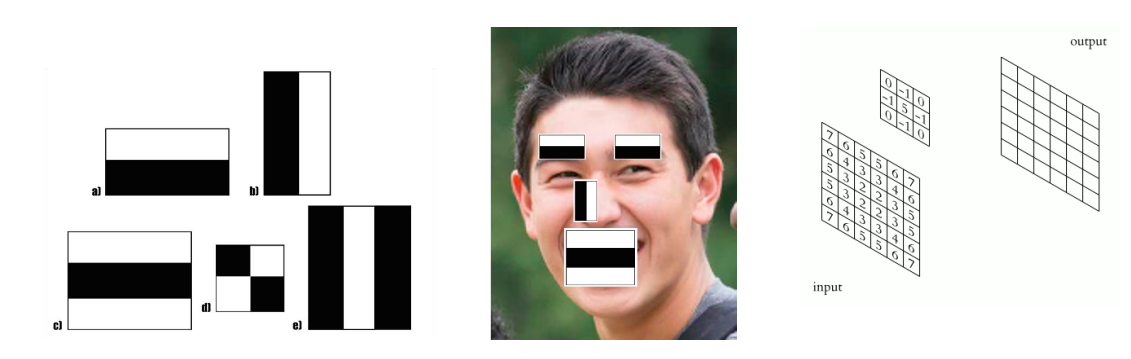
\includegraphics[height=4.3cm,keepaspectratio]{haar_cascade.png}
            \vspace{1mm}
            \begin{itemize}
                \item Haar Cascade phát hiện nhanh khuôn mặt frontal.
                \item Nếu có nhiều mặt, giữ bounding box lớn nhất.
            \end{itemize}
        \end{column}
        \begin{column}{0.48\textwidth}
            \centering
            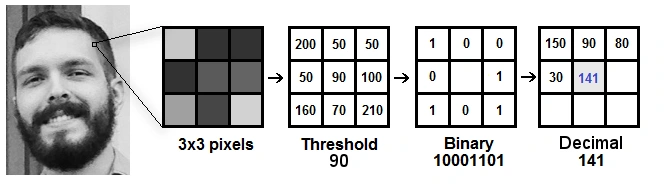
\includegraphics[height=4.3cm,keepaspectratio]{lbph.png}
            \vspace{1mm}
            \begin{itemize}
                \item LBPH nhận diện bằng khoảng cách histogram texture cục bộ.
                \item Ngưỡng nhận diện: \code{confidence < 150.0}.
            \end{itemize}
        \end{column}
    \end{columns}
\end{frame}

\begin{frame}{Đặc trưng đầu vào cho fuzzy}
    \begin{columns}[T]
        \begin{column}{0.32\textwidth}
            \begin{block}{Model confidence}
                Scale từ khoảng cách LBPH:
                \[
                    C=\max(0,100-\frac{70d}{150})
                \]
            \end{block}
        \end{column}
        \begin{column}{0.32\textwidth}
            \begin{block}{Illumination}
                Trung bình pixel grayscale trong ROI khuôn mặt.
            \end{block}
        \end{column}
        \begin{column}{0.32\textwidth}
            \begin{block}{Facial angle}
                Ước lượng từ bất đối xứng sáng giữa hai nửa ROI.
            \end{block}
        \end{column}
    \end{columns}

    \vspace{4mm}
    \begin{itemize}
        \item Các đặc trưng này giúp hệ thống phân biệt mặt rõ, mặt thiếu sáng và mặt quay lệch.
        \item Khi không có detection hoặc danh tính là \code{Unknown}, hệ thống xử lý theo hướng fail-safe.
    \end{itemize}
\end{frame}

\begin{frame}{Fuzzy logic decision}
    \begin{columns}[T]
        \begin{column}{0.55\textwidth}
            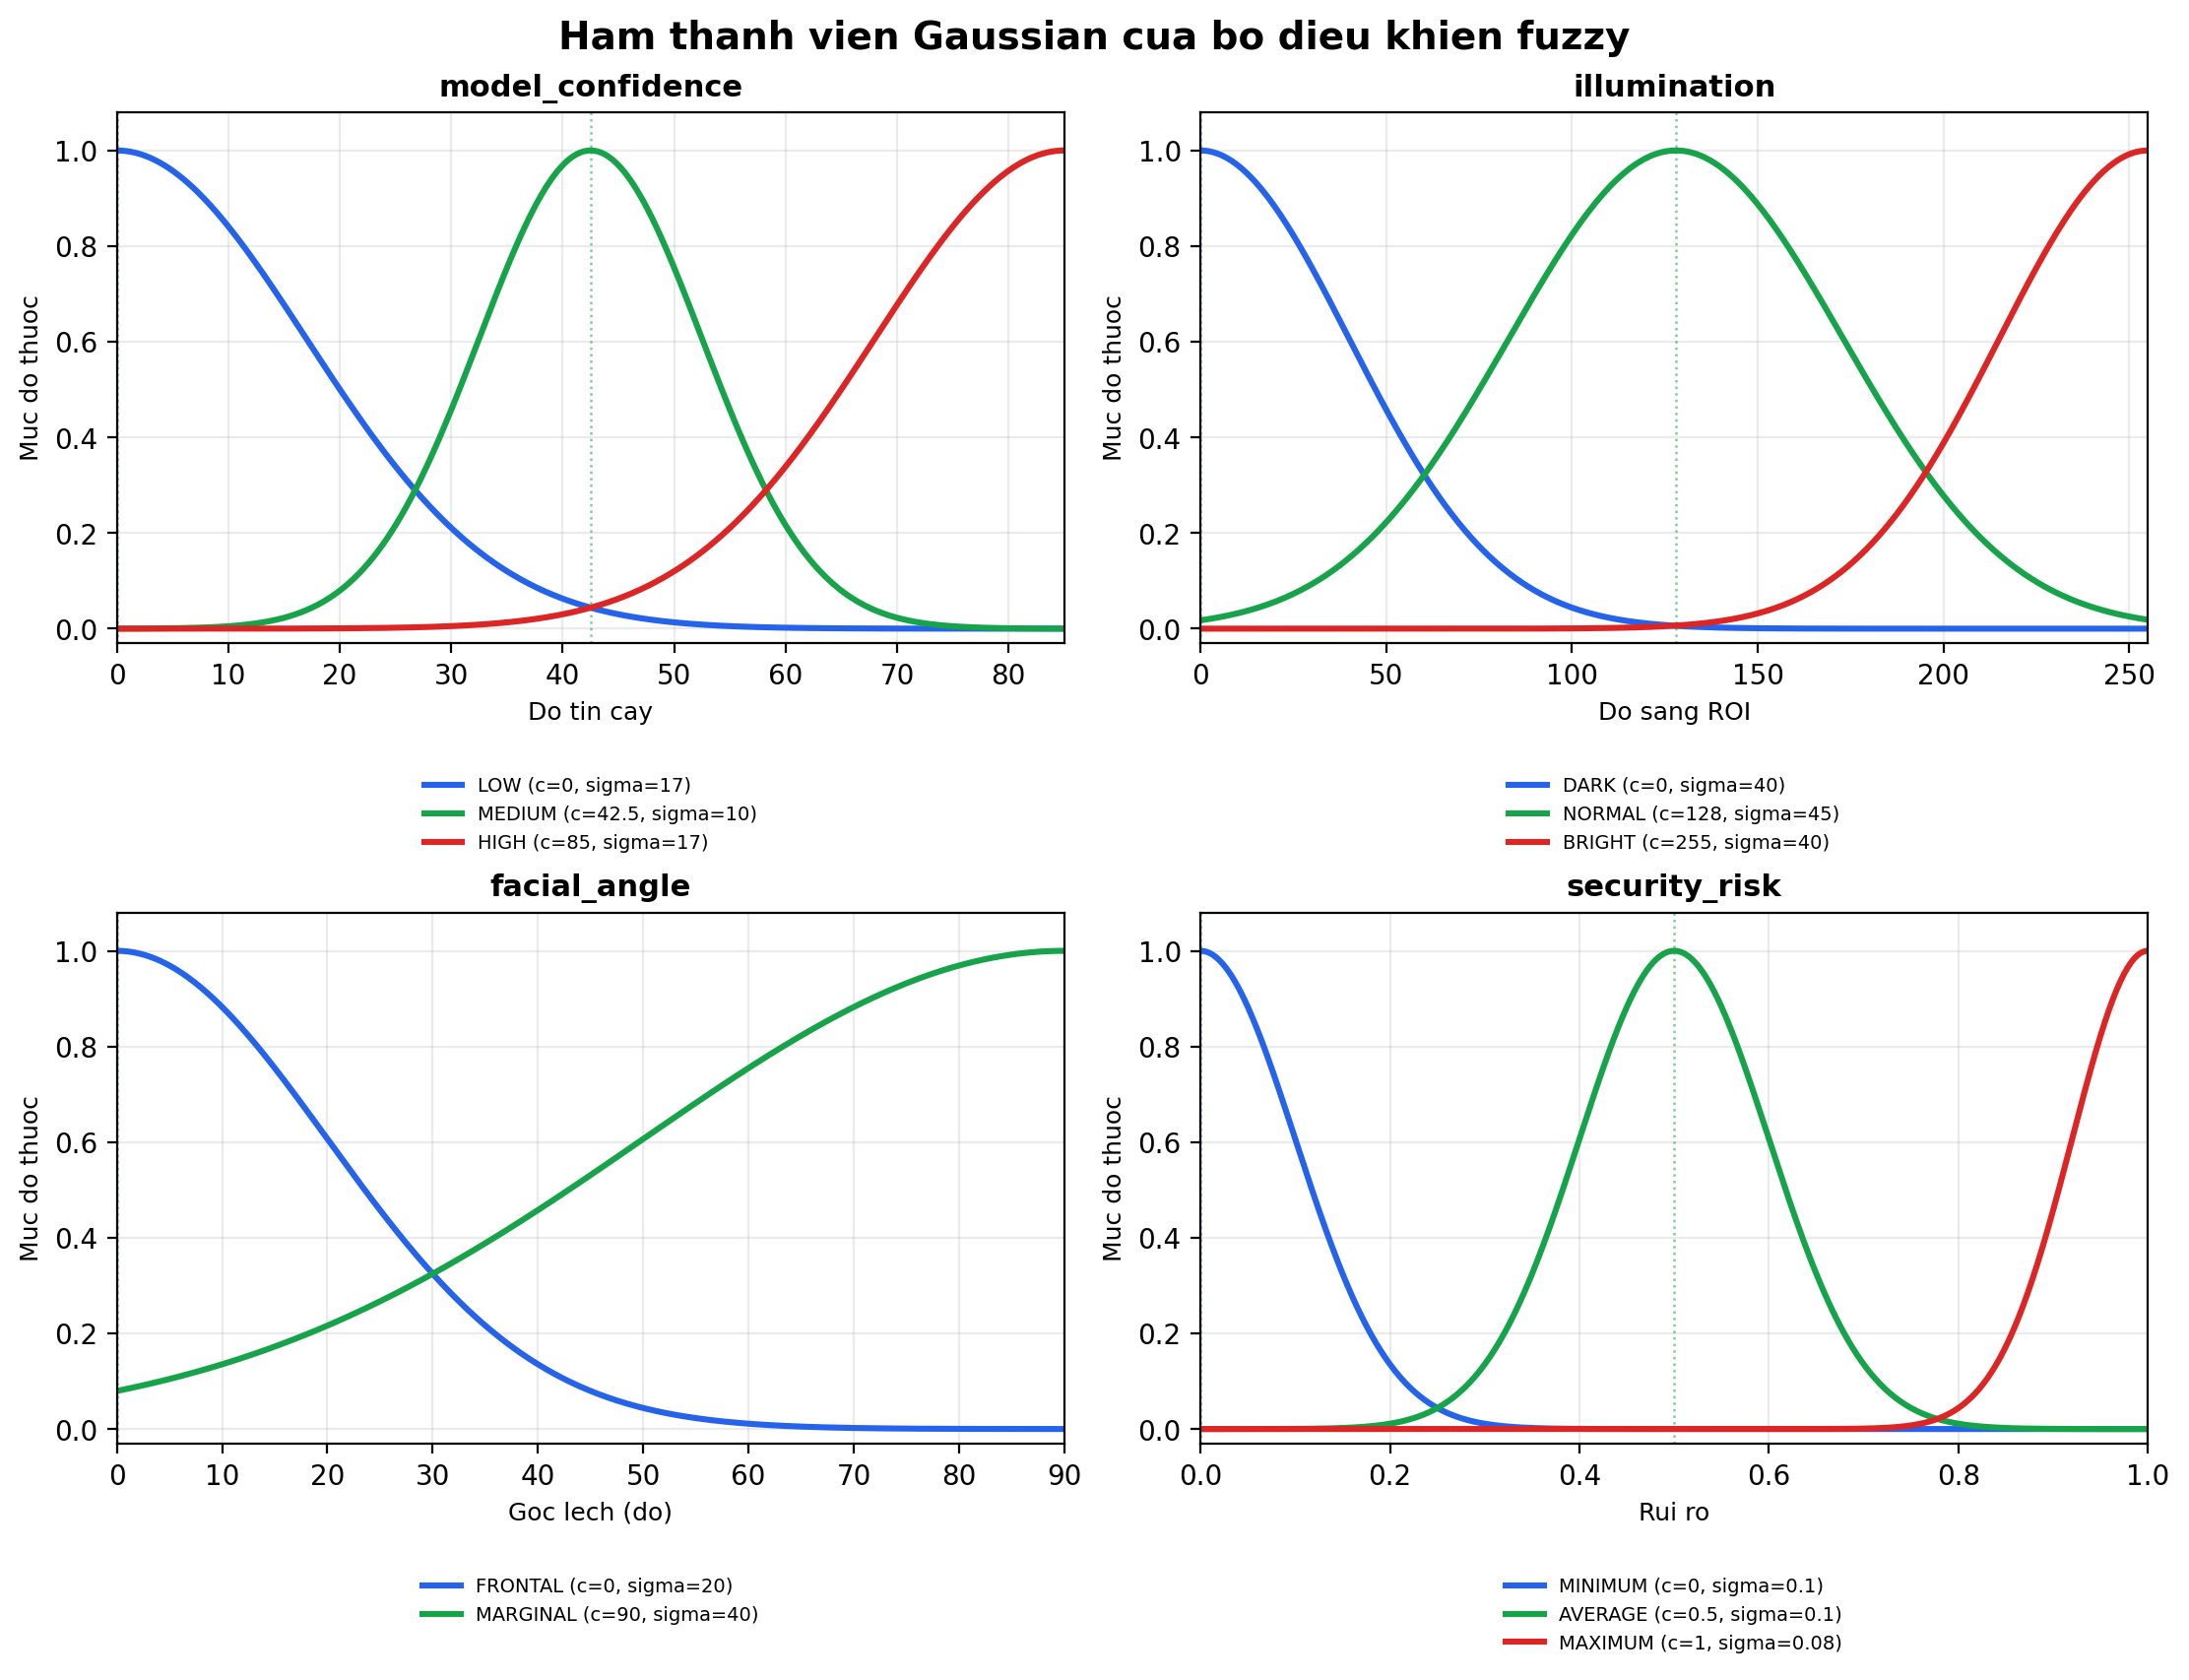
\includegraphics[width=\linewidth]{fuzzy_full.png}
        \end{column}
        \begin{column}{0.42\textwidth}
            \begin{itemize}
                \item Engine Mamdani với 3 input và 1 output.
                \item Hàm thành viên Gaussian cho confidence, illumination, angle và risk.
                \item AND dùng \code{Minimum()}, aggregation dùng \code{Maximum()}.
                \item Defuzzification bằng \code{Centroid(200)}.
            \end{itemize}
        \end{column}
    \end{columns}
\end{frame}

\begin{frame}{Luật fuzzy và ánh xạ hành động}
    \begin{columns}[T]
        \begin{column}{0.52\textwidth}
            \begin{block}{Nguyên tắc luật}
                \begin{itemize}
                    \item LOW confidence luôn dẫn tới MAXIMUM risk.
                    \item HIGH confidence chỉ an toàn khi ánh sáng NORMAL và mặt FRONTAL.
                    \item MEDIUM confidence cần điều kiện ảnh tốt, nếu không rủi ro tăng mạnh.
                \end{itemize}
            \end{block}
        \end{column}
        \begin{column}{0.43\textwidth}
            \begin{table}
                \centering
                \small
                \begin{tabular}{@{}ll@{}}
                    \toprule
                    \textbf{Security risk} & \textbf{Action}\\
                    \midrule
                    $<0.30$ & \code{unlock}\\
                    $<0.60$ & \code{otp}\\
                    $<0.85$ & \code{deny}\\
                    $\ge 0.85$ & \code{lockout}\\
                    \bottomrule
                \end{tabular}
            \end{table}
        \end{column}
    \end{columns}
\end{frame}

\begin{frame}{Thiết kế phần cứng}
    \begin{columns}[T]
        \begin{column}{0.48\textwidth}
            \small
            \begin{tabular}{@{}lll@{}}
                \toprule
                \textbf{Thiết bị} & \textbf{Chức năng} & \textbf{GPIO}\\
                \midrule
                Keypad 4x4 & Row 1--4 & 17, 27, 22, 5\\
                Keypad 4x4 & Col 1--4 & 6, 13, 19, 26\\
                Servo & PWM signal & 18\\
                OLED SPI & DC, RST & 24, 25\\
                OLED SPI & MOSI, SCLK, CE0 & 10, 11, 8\\
                \bottomrule
            \end{tabular}

            \vspace{4mm}
            \begin{itemize}
                \item Keypad quét bằng interrupt trên cột.
                \item Servo dùng PWM và duty về 0 sau khi quay.
                \item Servo dùng nguồn 5V ngoài, nối GND chung với Pi.
            \end{itemize}
        \end{column}
        \begin{column}{0.49\textwidth}
            \centering
            \resizebox{\linewidth}{!}{%
            \begin{tikzpicture}[
                >=Stealth,
                font=\scriptsize,
                pi/.style={draw, rounded corners, fill=green!8, minimum width=2.6cm, minimum height=4.4cm, align=center},
                dev/.style={draw, rounded corners, fill=blue!7, minimum width=2.6cm, minimum height=0.75cm, align=center},
                pwr/.style={draw, rounded corners, fill=red!7, minimum width=2.6cm, minimum height=0.75cm, align=center},
                wire/.style={thick, -{Stealth}},
                sig/.style={thick, blue!70!black, -{Stealth}},
                power/.style={thick, red!70!black, -{Stealth}},
                gnd/.style={thick, black!75, -{Stealth}}
            ]
                \node[pi] (pi) at (0,0) {\textbf{Raspberry Pi 4B}\\GPIO + USB};
                \node[dev] (cam) at (-3.6,1.8) {USB Camera};
                \node[dev] (keypad) at (3.6,1.7) {Keypad 4x4};
                \node[dev] (oled) at (3.6,0.2) {OLED SSD1306};
                \node[dev] (servo) at (3.6,-1.3) {RC Servo};
                \node[pwr] (supply) at (-3.6,-1.8) {Nguồn 5V ngoài};
                \draw[wire] (cam.east) -- (pi.west);
                \draw[sig] (pi.east) -- (keypad.west);
                \draw[sig] (pi.east) -- (oled.west);
                \draw[sig] (pi.east) -- (servo.west);
                \draw[power] (supply.east) -- (servo.west);
                \draw[gnd] (supply.north east) to[bend left=15] (pi.south west);
            \end{tikzpicture}}
        \end{column}
    \end{columns}
\end{frame}

\begin{frame}{Mạch đấu nối thực tế}
    \begin{columns}[T]
        \begin{column}{0.62\textwidth}
            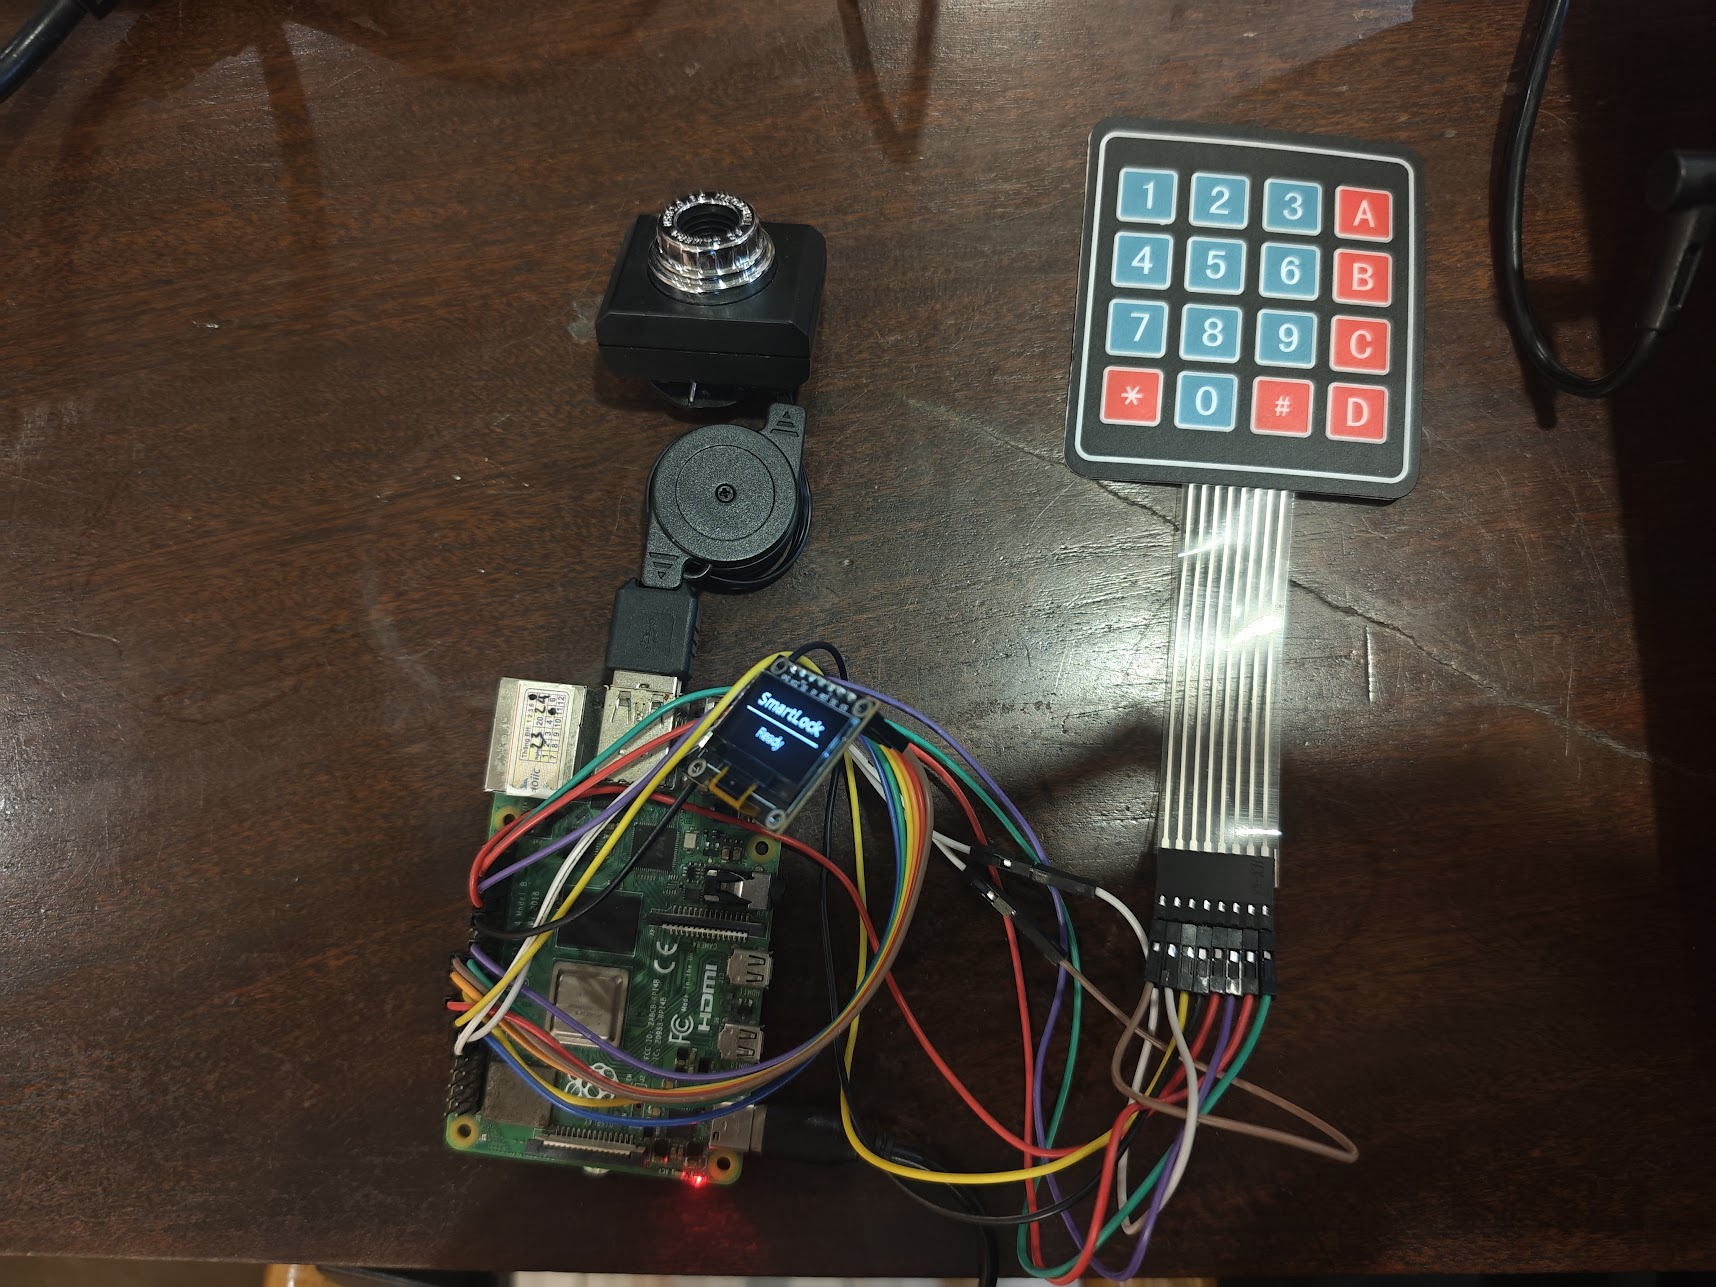
\includegraphics[width=\linewidth]{schematic_connected.png}
        \end{column}
        \begin{column}{0.35\textwidth}
            \begin{itemize}
                \item Raspberry Pi 4B là thiết bị edge chính.
                \item Camera USB phục vụ nhận diện.
                \item Keypad dùng xác thực PIN dự phòng.
                \item OLED hiển thị trạng thái hệ thống.
                \item Servo mô phỏng cơ cấu chốt khóa.
            \end{itemize}
        \end{column}
    \end{columns}
\end{frame}

\begin{frame}{Dashboard web}
    \begin{columns}[T]
        \begin{column}{0.64\textwidth}
            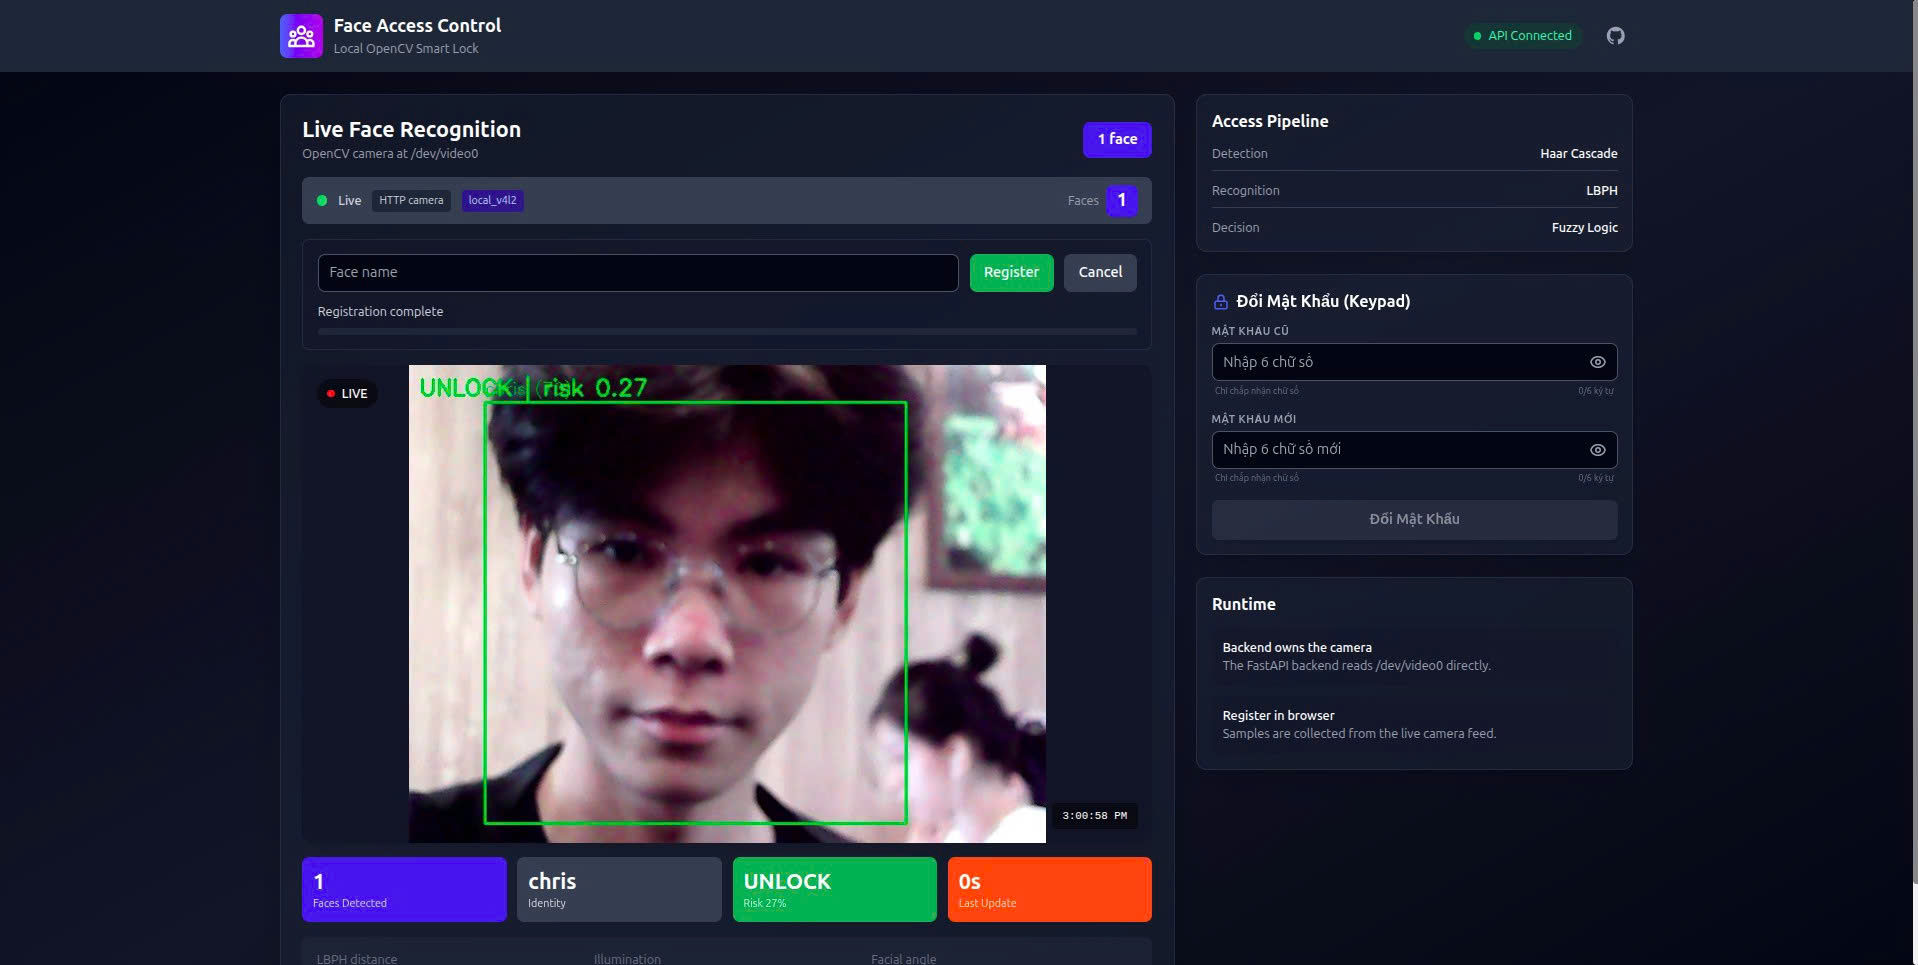
\includegraphics[width=\linewidth]{dashboard_nextjs.png}
        \end{column}
        \begin{column}{0.33\textwidth}
            \begin{itemize}
                \item Polling \code{/api/v1/camera/frame}.
                \item Hiển thị live frame, identity, LBPH distance, illumination, facial angle.
                \item Đăng ký khuôn mặt và đổi mã PIN từ giao diện web.
            \end{itemize}
        \end{column}
    \end{columns}
\end{frame}

\begin{frame}{Benchmark trên dashboard}
    \begin{columns}[T]
        \begin{column}{0.64\textwidth}
            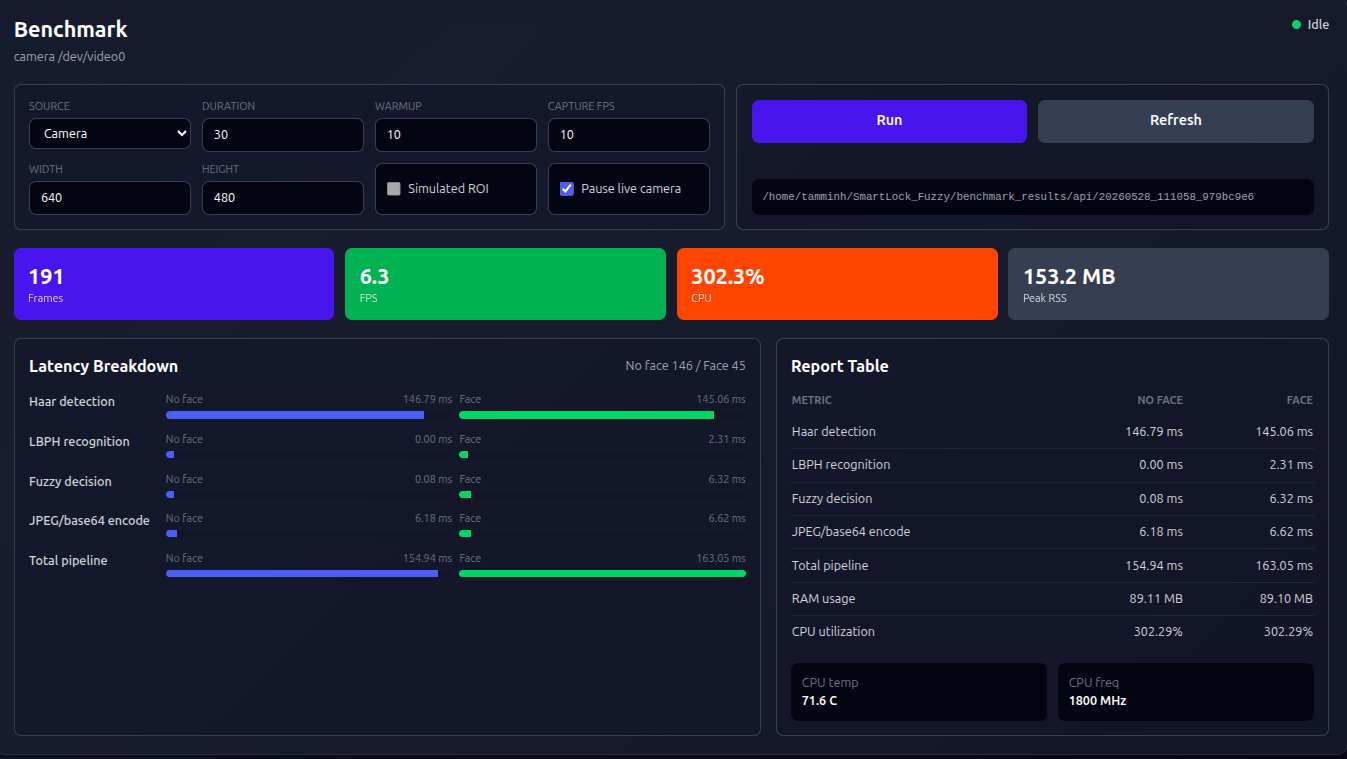
\includegraphics[width=\linewidth]{benchmark_ui.png}
        \end{column}
        \begin{column}{0.33\textwidth}
            \begin{itemize}
                \item Frontend có panel Benchmark để chạy và xem kết quả đo.
                \item Backend ghi \code{summary.json}, \code{summary.md}, \code{frames.csv}.
                \item Các metric chính: FPS, CPU, RAM, nhiệt độ, latency từng bước.
            \end{itemize}
        \end{column}
    \end{columns}
\end{frame}

\begin{frame}{Kết quả benchmark trên Raspberry Pi}
    \begin{columns}[T]
        \begin{column}{0.24\textwidth}
            \begin{block}{Tổng quan}
                \centering
                \metric{489}{frame đo}\\[3mm]
                \metric{60.05 s}{thời gian}\\[3mm]
                \metric{8.14 FPS}{throughput}
            \end{block}
        \end{column}
        \begin{column}{0.72\textwidth}
            \small
            \begin{tabular}{@{}lcc@{}}
                \toprule
                \textbf{Chỉ số} & \textbf{Không có mặt} & \textbf{Có mặt}\\
                \midrule
                Face detection latency & 111.26 ms & 108.43 ms\\
                Face recognition latency & 0.00 ms & 2.15 ms\\
                Fuzzy decision latency & 0.08 ms & 5.90 ms\\
                JPEG/base64 encode latency & 5.91 ms & 6.34 ms\\
                Total pipeline latency & 121.36 ms & 127.36 ms\\
                RAM usage & 89.27 MB & 89.25 MB\\
                CPU utilization & 319.07\% & 319.07\%\\
                \bottomrule
            \end{tabular}

            \vspace{3mm}
            \begin{itemize}
                \item Haar Cascade là bước chiếm thời gian lớn nhất.
                \item Nhiệt độ cuối: $67.7^\circ$C, CPU 1800 MHz, throttling \code{0x0}.
            \end{itemize}
        \end{column}
    \end{columns}
\end{frame}

\begin{frame}{Đánh giá}
    \begin{columns}[T]
        \begin{column}{0.49\textwidth}
            \begin{block}{Kết quả đạt được}
                \begin{itemize}
                    \item Backend, frontend và phần cứng đã chạy thành một hệ thống hoàn chỉnh.
                    \item Fuzzy logic giúp quyết định dựa trên cả danh tính và chất lượng frame.
                    \item Benchmark cho thấy độ trễ khoảng 127 ms khi có khuôn mặt.
                \end{itemize}
            \end{block}
        \end{column}
        \begin{column}{0.49\textwidth}
            \begin{block}{Giới hạn}
                \begin{itemize}
                    \item LBPH nhạy với ánh sáng và dữ liệu đăng ký.
                    \item Facial angle mới là ước lượng tương đối.
                    \item API quản trị và PIN runtime cần cơ chế bảo mật/lưu bền vững hơn.
                \end{itemize}
            \end{block}
        \end{column}
    \end{columns}
\end{frame}

\begin{frame}{Kết luận và hướng phát triển}
    \begin{itemize}
        \item Đề tài hiện thực một khóa cửa thông minh chạy cục bộ trên Raspberry Pi, gồm nhận diện khuôn mặt, fuzzy decision, keypad, OLED, servo và dashboard web.
        \item Kết quả benchmark cho thấy pipeline đủ dùng cho kịch bản khóa cửa, nơi yêu cầu phản hồi ổn định dưới một giây.
        \item Hướng phát triển: thay LBPH bằng face embedding nhẹ hơn, thêm xác thực API, lưu PIN/log bằng SQLite, tăng test tự động và tối ưu face detection.
    \end{itemize}

    \vspace{7mm}
    \begin{center}
        \Large Cảm ơn thầy và các bạn đã lắng nghe.
    \end{center}
\end{frame}

\end{document}
